\chapter{Implementation}
\label{chap:implementation}

The QAOA algorithm is very reliant on finding appropriate angles $(\vec{\gamma},\vec{\beta})$ that favour good partitions and causes bad partitions to destructively interfere. One of the main obstacles to overcome is determining those optimal angles efficiently. In \cite{ZWCPL18} two methods were proposed to tackle this problem, INTERP and FOURIER that run in poly$(p)$ time. In this chapter, I will discuss the INTERP method together with the practical intricacies of implementing QAOA.
\\~\\
All the code developed for this thesis can be found on my GitHub repository: $\ $    \url{https://github.com/soosub/bep/} in the folder \code{Implementation/NewPlan}

\section{Patterns in the optimal parameters}

In order to improve upon current methods, extensive searches for globally optimal angles were conducted in \cite{ZWCPL18, Crooks18}  and independently found interesting results. After degeneracies were reduced from the parameter space, there were patterns to be found relating the optimal parameters for a particular graph at level $p$ to the optimal parameters at level $p+1$, as shown in Figure \ref{fig:patterns-zhou}.

\begin{figure}[H]
	\centering
	\begin{subfigure}[t]{0.5\textwidth}
		\centering
		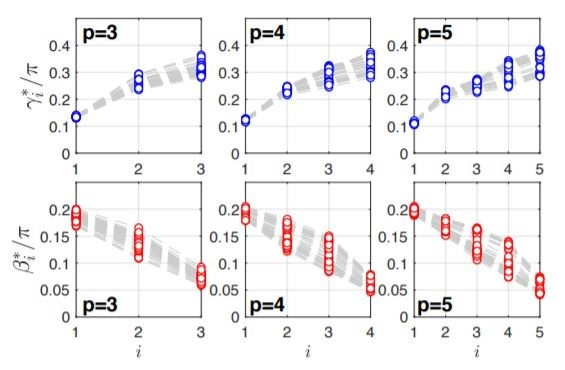
\includegraphics[width=\textwidth]{figures/patterns-u3R.jpg}
		\caption{Optimal parameters for unweighted 3-regular graphs}
	\end{subfigure}%
	~ 
	\begin{subfigure}[t]{0.5\textwidth}
		\centering
		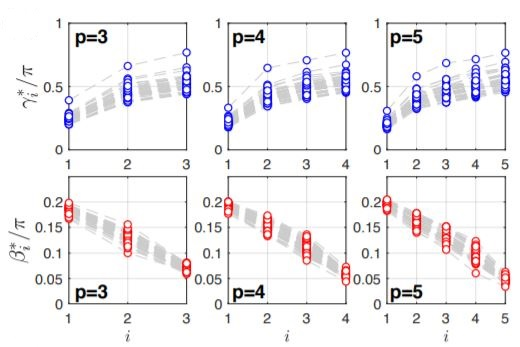
\includegraphics[width=\textwidth]{figures/patterns-w3R.jpg}
		\caption{Optimal parameters for weighted 3-regular graphs}
	\end{subfigure}
	\caption{ The parameter pattern visualized by plotting the optimal parameters of 40 instances of 16-vertex unweighted 3 regular graphs (a) and 16-vertex weighted 3 regular graphs (b), for $3 \leq p \leq 5$. The weights $w_{ij}$ in the weighted graphs were chosen from a uniform distribution $[0, 1]$. Each dashed line connects parameters for one particular graph instance. For each instance and each $p$, the classical BFGS optimization routine was used from $10^4$ random initial points, and the best parameters were kept. Figure and results from \cite{ZWCPL18}.}
	\label{fig:patterns-zhou}
\end{figure} 
\newpage
Independently, similar patterns were found on 10 node graphs in \cite{Crooks18}, see Figure \ref{fig:patterns-crooks}.

\begin{figure}[H]
	\centering
	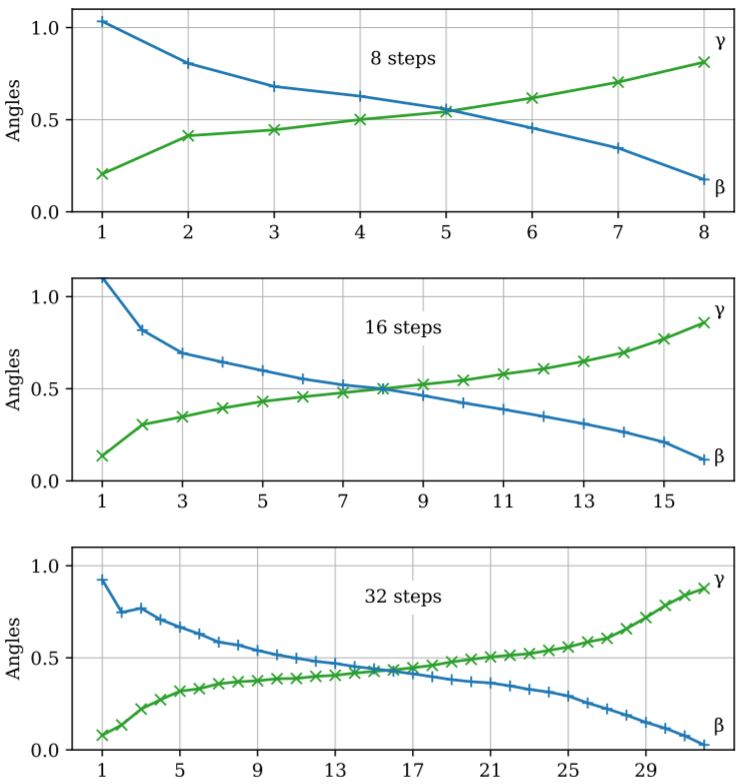
\includegraphics[scale=0.5]{figures/patterns-crooks.jpg}
	\caption{Examples of optimized parameters $(\vec{\beta}_{\text{opt}}, \vec{\gamma}_{\text{opt}})$ for Max-Cut QAOA on 10 node graphs, with 8, 16, and 32 QAOA	steps. The graph was chosen from the Erd\H{o}s-R\'enyi ensemble with edge probability 50\%.  When comparing with Figure \ref{fig:patterns-zhou}, there is a difference in the scaling of the $\beta_i$ parameters, this is because \cite{Crooks18} used the mixer Hamiltonian $H_B = \frac{1}{2}\sum_j \sigma_x^{(j)}$ whereas \cite{ZWCPL18} used the mixer Hamiltonian $H_B = \sum_j \sigma_x^{(j)}$, resulting in a factor 2 difference. Figure and results from \cite{Crooks18}.}
	\label{fig:patterns-crooks}
\end{figure}

As one can see from both results, $\gamma_i$ is a monotonically increasing sequence while $\beta_i$ is a monotonically decreasing sequence, for $i \in \{1, \dots p\}$. This is reminiscent of the Quantum Adiabatic Algorithm using a linear annealing schedule, where the initial Hamiltonian is turned off gradually while the final, or problem Hamiltonian is turned on \cite{AL18}. In addition, the optimal parameters found in $p$-level QAOA are very similar to the optimal parameters in the next level. This opens up the possibility of exploiting this relation in order to speed-up the parameter determination as will be discussed in Section \ref{sec:proposed-methods}.
	
\section{Proposed method by Zhou et al.}
\label{sec:proposed-methods}
In \cite{ZWCPL18}, it was suggested to use the patterns they found in order to enhance the search for optimal parameters. Two methods were proposed to achieve this, namely INTERP and FOURIER. Both methods require poly($p$) time, as opposed to, for example, gridsearch. The general idea in both methods is to use the optimal, or quasi-optimal angles at level $p$, and make an educated guess for the initial point of the optimization routine for the next level $p+1$. In the next section I will focus on the INTERP method.

\subsection{INTERP}
INTERP uses linear interpolation to produce a good initial point $(\vec{\gamma},\vec{\beta})$ for optimising the QAOA parameters as one iteratively increases the level $p$

\begin{equation}
\Big[\vec{\gamma}_{(p+1)}^0\Big]_i = \frac{i-1}{p}\Big[\vec{\gamma}_{(p)}^L\Big]_{i-1} + \frac{p-i+1}{p}\Big[\vec{\gamma}_{(p)}^L\Big]_i
\end{equation}
\begin{equation}
\Big[\vec{\beta}_{(p+1)}^0\big]_i = \frac{i-1}{p}\Big[\vec{\beta}_{(p)}^L\Big]_{i-1} + \frac{p-i+1}{p}\Big[\vec{\beta}_{(p)}^L\Big]_i
\end{equation}
for $i = 1, 2, \dots, p+1$. Here, the superscript indicates either that the angle pertains to the local minimum, $L$, or that it is the initial point for the next optimization round. The subscript inside the brackets indicates the QAOA level, and the subscript outside the brackets indicates the array element. Since the notation might seem a bit daunting, consider the following example. Suppose we have a (local optimal) set $\vec{\gamma}^L_{(3)} = (\gamma_1, \gamma_2,\gamma_3)$ for $p=3$ found after some optimization routine. Then, we can find a good initial point $\vec{\gamma}^0_{(4)} = (\gamma_1^0, \gamma_2^0,\gamma_3^0, \gamma_4^0)$ using the INTERP method for $p=4$ using these parameters, see Figure \ref{fig:interp-example}.
\begin{figure}[H]
	\centering
	\begin{subfigure}[t]{0.45\textwidth}
	\centering
	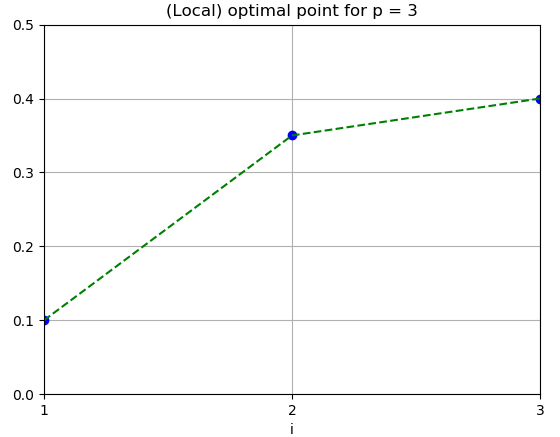
\includegraphics[width=\textwidth]{figures/heuristic_optimal_params.png}
	\end{subfigure}%
	~
	\begin{subfigure}[t]{0.45\textwidth}
		\centering
		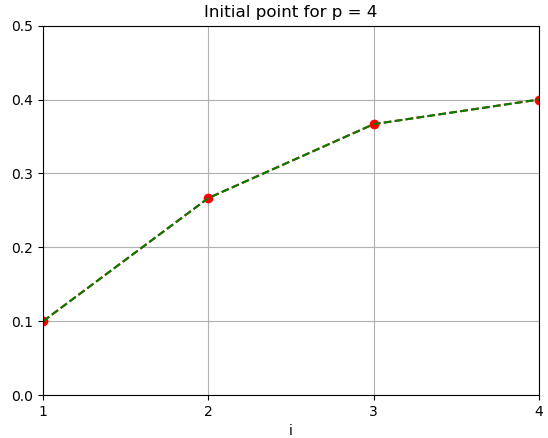
\includegraphics[width=\textwidth]{figures/heuristic_initial_params.png}
	\end{subfigure}%
	\caption{Illustration of INTERP method. The method uses the (local) optimal parameters to derive a good initial point for the optimization round of the next layer, using interpolation.}
	\label{fig:interp-example}
\end{figure}
Note that the parameters found using this interpolation are used as \emph{initial point} for the next round of optimization, so these are not directly the parameters used in the circuit. From this initial point we start another round of optimization to find a local optimum, that hopefully is also the global minimum or close to it. This is accomplished by considering the expectation value $\langle H_C \rangle$ as our objective function, which is estimated by sampling multiple times from the state $|\gambe\rangle$ and then calculating the corresponding objective value. When the next local minimum is found we use it to generate angles for the next $p$, and in this fashion we iteratively increase $p$ untill we are satisfied.

In some sense, it is flexible as one is not obliged to start from $p=1$, but can start at any level $p_{0}$ given an initial set of angles $\gamma_1, \beta_1 \dots \gamma_{p_{0}}, \beta_{p_{0}}$. For Max-Cut, it was recommended by Zhou to start from $p_0=1$ with $(\gamma, \beta) = (0.8,0.35)$ as an initial guess and work from there \cite{Zhou-email, genQAOA}. This is the approach I will use when producing the results in the next chapter. Alternatively, one could choose to do a gridsearch for the first layer requiring $O(1)$ function calls, and then proceed using INTERP.

%\section{Particle Swarm Optimization}
%In addition to the methods proposed in \cite{ZWCPL18}, I also tried out Particle Swarm Optimization (PSO) \cite{PSO1, PSO2} for parameter optimization. PSO is a gradient-free, evolutionary optimization approach that has been succesfully applied to many problems such as artificial neural network training, function optimization, and pattern classification \cite{Engelbrecht06,Poli08}. This was implemented using the package pySwarm \cite{pyswarm}. Applying PSO optimization to QAOA lead to some promising results in \cite{QAOA-pso}.

\section{Number of samples}
One algorithm design choice to consider is the number of samples from $|\gambe\rangle$ one needs when determining the final answer. Taking a constant number of samples would naturally lead to poor performance for large graphs, as the number of possible partitions grows exponentially with $n$. Another (naieve) option would be to take a certain fraction of the possible number of partitions, but asymtotically this would require $O(2^n)$ function calls. Ideally, we want to bound the number of samples by a polynomial function of $n$ and still get results close to or better than $F_p = \langle H_C \rangle$. It turns out we can. Remember from equation \eqref{eq:concentration} that the variance is bounded which implied that for fixed $p$ and $v$ the sample mean of order $m^2$ values of $C(\mathbf{z})$ will be in $[F_p(\gambe)-1,F_p(\gambe)+1]$ with probability $1 - \frac{1}{m}$ \cite{FGG14}. This means for reasonably large graphs ($m \gtrsim 10$), we can simply take $m^2$ samples and still find our estimate to be between $F_p \pm 1$ with reasonable probability. An illustration of the necessary $F_p$ evaluations as a fraction of the total number of partitions is shown in Figure \ref{fig:fraction}.

One thing to notice is that this impairs the applicability of QAOA for small graphs. The algorithm is inherently stochastic and so it requires multiple samples from the state $|\gambe\rangle$. When the number of samples required exceeds the number of possible partitions $2^n$ this nullifies the benefits of using the algorithm, even if we know good angles beforehand. Note that this fraction is based on \emph{one} evaluation of $F_p$. If, in addition, we still need to find good or optimal angles using classical optimization in the outer loop, then the number of necessary $F_p$-evaluations could diminish the usefulness of QAOA. Moreover, if one chooses to use a VQE subroutine for determining optimal angles it is likely that one would need more samples per function call since an unaccurate expectation estimate could restrain the effectiveness of the optimization when looking for (local) minima.

\begin{figure}[H]
	\centering
	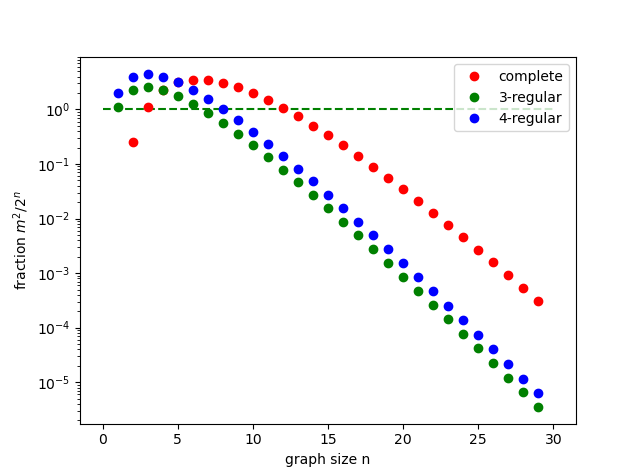
\includegraphics[width=0.58\textwidth]{figures/fraction.png}
	\caption{The ratio of necessary samples $m^2$ for finding a reasonalbe estimate for $\langle H_C \rangle$ and the total number of possible partitions $2^n$ as a function of the graph size $n$, here $m$ denotes the number of edges in the graph. With a reasonable estimate I mean that we find $F_{p, \text{sampled}}$ within 1 of the actual $F_p$ with a $1-\frac{1}{m}$ probability. The figure shows complete, 3-regular and  4-regular graphs. Note that for small complete graphs brute force approaches are superior to QAOA as one would need more samples then there are possible partitions to accurately estimate $F$.}
	\label{fig:fraction}
\end{figure}


\section{Implementation in Python}
\subsection{QAOA and Goemans-Williamson}
In order to examine the INTERP method, I implemented it using Python. For simulating the quantum circuit that is shown in Figure \ref{fig:schematic-qaoa}, I used pyQuil \cite{pyQuil}. pyQuil is a quantum instruction language developed at Rigetti Computing. It provides a way to simulate and compile quantum programs. The Quantum Virtual Machine (QVM) was used to run my experiments. Moreover, I made use of Grove, a collection of quantum algorithms built using the Rigetti Forest platform. Grove provides an implementation of QAOA using the VQE subroutine, on top of which I build the INTERP method. This was achieved by running the QAOA circuit for a certain set of initial angles to find a local minimum, which is illustrated in Figure \ref{fig:schematic-qaoa-vqe}. This local minimum was then used to calculate a new set of initial angles for the next QAOA layer according to the INTERP scheme. The optimizer used in the VQE subroutine was BFGS \cite{BFGS}. The quantum parts were simulated using the QVM and perfect qubits and full connectivity were assumed. The expectation $F_p$ was calculated during the optimization rounds using a fast method by dotting the wavefunction with the objective operator \cite{pyQuil}.

To benchmark the INTERP method to other QAOA methods, I also analyzed the performance of QAOA when starting from randomly chosen initial points, again with the Grove's QAOA class. I will abbreviate this method to pyQuil RI (randomly intialised), or simply RI. This means that for a given $p$, the optimization is simply started from $\vec{\gamma} = (\gamma_1,...,\gamma_p)$ and $\vec{\beta} = (\beta_1,...,\beta_p)$ with $\gamma_i$ drawn from a uniform distribution $U[0,2\pi]$ and $\beta_i$ from a uniform distribution $U[0,\pi]$. Again I used a BFGS optimizer in the VQE subroutine.

I used the implementation of the Goemans-Williamson algorithm from the package cvxgraphalgs. 

\subsection{Graphs}
The graphs that were analyzed were generated using the Python package networkx \cite{networkx}, a Python package for the creation, manipulation, and study of graphs and complex networks. These graphs include cyclic graphs, 3-regular graphs and weighted 3-regular graphs, and graphs from the Erd\"os-R\'enyi ensemble with edge probabilities 0.5, and 0.75. To make sure the experiments done are reproducable, I used seeds to keep track of the randomly generated graphs, the 3-regular graphs and the Erd\"os-R\'enyi graphs. For the regular graphs, I used a seed ranging from 0 to $N$, where $N$ is the number of graphs analyzed for that particular class of graphs. The same was done for the Erd\"os-R\'enyi (ER) graphs, however for small graphs and low edge probability there is a small probability that there are no edges in the graph. To circumvent this, I simply used the condition that the set of edges had to be non-empty, and if it were empty skip to the next seed.\\

Python version 3.7.7 was used. Relevant software and Python packages with corresponding versions are included in Appendix \ref{appendix:packages}.
